\documentclass{beamer}

\mode<presentation>
{
  \usetheme{Warsaw}
  % or ...

  \setbeamercovered{transparent}
  % or whatever (possibly just delete it)
}


\usepackage[english]{babel}
% or whatever

\usepackage[utf8]{inputenc}
% or whatever

\usepackage{times}
\usepackage[T1]{fontenc}
% Or whatever. Note that the encoding and the font should match. If T1
% does not look nice, try deleting the line with the fontenc.


\title{Simulation of the Nomification of Independent Chord Rings}
\author{Andrew Rosen \qquad Brendan Benshoof }
\date{} % Activate to display a given date or no date (if empty),
         % otherwise the current date is printed 
         


% If you wish to uncover everything in a step-wise fashion, uncomment
% the following command: 

%\beamerdefaultoverlayspecification{<+->}


\begin{document}

\begin{frame}
  \titlepage
\end{frame}

\begin{frame}{Outline}
  \tableofcontents
  % You might wish to add the option [pausesections]
\end{frame}

\section{Goals of Modeling and Simulation}

\subsection{Problem Space}

\begin{frame}{File Lookup}
	\begin{itemize}
		\item Most important function of a decentralized Peer-to-Peer system.
		\item Need to discover which node in the network has a certain file.
		\item Need to do it efficiently.
	\end{itemize}

\end{frame}


\begin{frame}{Hashing Protocols}
	\begin{itemize}
		\item One of the best solutions for this task.
		\item Map nodes and files identifiers to keys.
		\item Nodes are responsible for files with keys that match some criteria,.
		\item Imposes an structure on the network.
	\end{itemize}

\end{frame}


\subsection{Chord}

\begin{frame}{What is Chord}
	\begin{itemize}
		\item Arranges a network into a ring.
		\item Maximum $2^m$ nodes in the network.
		\item Nodes and filenames are hashed to create an $m$-bit key.
	\end{itemize}

\end{frame}

\begin{frame}{How Are Files Stored}
\begin{center}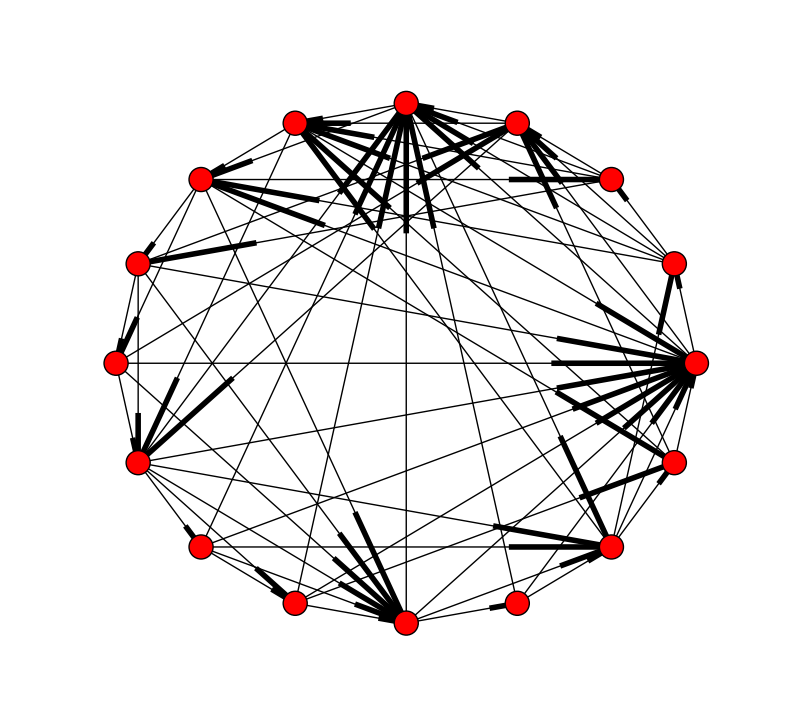
\includegraphics[scale=0.25]{chordreal}\end{center}
	\begin{itemize}
		\item Node responsible for for key $\kappa$ is the $sucessor(\kappa)$.
		\item $sucessor(\kappa)$ is the node with key $\kappa$ or first following key.
	\end{itemize}

\end{frame}


\begin{frame}{How Are Files Retrieved}
	\begin{itemize}
		\item To find a file with key $\kappa$, we find $sucessor(\kappa)$.
		\item We could just ask our successor, who would do the same.
		\item We use a \emph{finger-table} make this quicker
		\begin{itemize}
			\item $m$ entries in the table.
			\item Stores location of $successor(n+2^{i-1})$ $mod$ $2^m$.
			\item If $\kappa$ is between us and an entry, skip to that entry.
		\end{itemize}
		\item Once we know $sucessor(\kappa)$, we can directly connect.
		\item This reduces the lookup time to $O(\log n)$
	\end{itemize}

\end{frame}


\begin{frame}{How Is Churn Handled}
	\begin{itemize}
		\item Join a network by asking some node in it to find your successor.
		\item Periodically update the entries in the finger table.
		\item Periodically find your successor's predecessor.
	\end{itemize}

\end{frame}

\subsection{Goals}
What happens:
\begin{frame}{Goals}
	\begin{itemize}
		\item If there is more than one initial ring?
		\item If our range of sight is limited?
		\item ANOTHER THING
		\item We ignore file lookup; identical to node lookup.
	\end{itemize}

\end{frame}



\section{Developed Models} 


\subsection{Agents}
\begin{frame}{Agents}
	\begin{itemize}
		\item Nodes for nodes, Links for links.
		\item Seekers.
		\item Updates.
	\end{itemize}
\end{frame}


\subsection{Simulation}

\begin{frame}{Setup}
	\begin{itemize}
		\item Generate nodes in random locations (ring visualization optional)
		\item Specified number of nodes for independent rings. 
		\item Set the hash size.
	\end{itemize}
\end{frame}

\subsection{Ouroboros Inaction}



\section{Experiments and Results}


\section{Conclusion and Future Work}

\begin{frame}{Stuff}

\end{frame}



\end{document}


